\chapter{Let's Get Started}
\label{ch:lgstarted}
% ##################################################################################################################
\hfill \textbf{Authors:} Andreas Horni, Kai Nagel, Marcel Rieser

\begin{center} 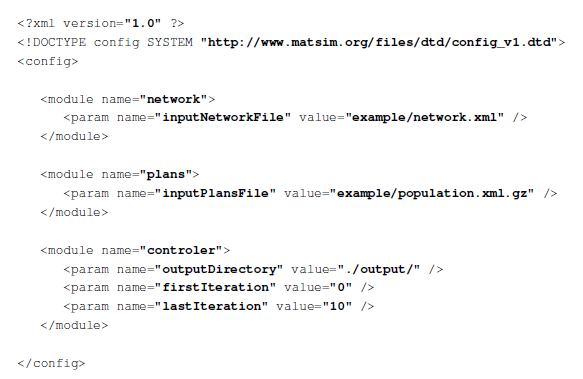
\includegraphics[width=0.7\textwidth, angle=0]{using/figures/config.png} \end{center}

% ##################################################################################################################
This chapter explains how to set up and run \gls{matsim} and it describes the requirements of building a basic \gls{scenario}. As this book tries to be as stable and timeless as possible, the \gls{matsim} user guide \citep[][]{MATSim_Userguide_2015} needs to be consulted in addition to this chapter for doing an actual installation; frequently changing and detailed information such as download paths or version-dependent configurations are omitted here as far as possible and left to the user guide. 

Getting the source code into different computing environments and extending \gls{matsim} through the \gls{api} is described in the second part of the book in Chapter~\ref{ch:extensionpoints}.

%% \kai{Ich würde bei den xml snippets gerne überall den header entfernen, überall eine Formulierung benuzten in etwa wie ``a minimal config file approximately looks as follows'', und überall zusätzlich eine stabile(!!) Referenz auf Versionen im Repository geben (muss noch schauen, wie wir das machen).  Z.B.\ ist config inzwischen bereits v2, und hat an manchen Stellen eine modernere Syntax; das fällt nur deshalb nicht auf, weil die alte Syntax noch überall akzeptiert wird.}

%% \ah{klingt gut.}

% ##################################################################################################################
\section{Running MATSim}
\label{sec:runningmatsim}

% ================================================================================================
\subsection{Setting Up MATSim}
\label{sec:settingUpMatsim}

To run \gls{matsim} you have to install the \gls{javase} that complies with the \gls{matsim} version to be run. At the time of writing this book, this is \gls{javase}~7.

Furthermore you need the official \emph{\gls{matsim} release,} which comes as a zip file (usually named with the version number \lstinline|matsim-yy.yy.yy.zip|) including everything that is required to run it. It can be downloaded following the ``release'' link under \url{http://matsim.org/downloads}.
%on the \gls{matsim} web page. 
Unzipping it results in the \textbf{\gls{matsim} directory tree}.   Continue with Section~\ref{sec:runexample}.

If you prefer to use the more up to date \emph{nightly builds,} you need to download
\begin{compactitem}
\item the \gls{matsim} \gls{jar} file (usually named with the revision number \lstinline|MATSim_ryyyy.jar|), and

\item the required external \glspl{library} (\lstinline|MATSim_libs.zip|). 

Unzipping this collection of 3rd-party libraries, you should then get a directory \lstinline|libs| with several \gls{jar} files inside. If the directory \lstinline|libs| is in the same directory as the \gls{matsim} \gls{jar} file, the libraries are found automatically and do not have to be added to the \lstinline|classpath| manually.
\end{compactitem}

% ================================================================================================
\subsection{Running MATSim}
\label{sec:runexample}

%% \kai{note: inzwischen kann man auch einfach auf das matsim jar draufklicken. :--)  Das sollten wir unbedingt nochmal testen, und dann beschreiben.  (Geht nicht mit dem derzeitigen release 6, aber im HEAD und nightly builds geht es schon.)}

%% \ah{hab den Text entsprechend angepasst.}

At the time of writing this book, the nightly built \gls{matsim} \gls{jar} file is executable by double-clicking. A minimal \gls{gui} as shown in Figure~\ref{fig:matsimgui} opens and the \gls{matsimrun} can be configured and started. 
This feature is expected to be in the releases starting with version 0.7.

% ----------
\createfigure[!h!]%
{Minimal MATSim GUI}%
{Minimal MATSim GUI}%
{\label{fig:matsimgui}}%
{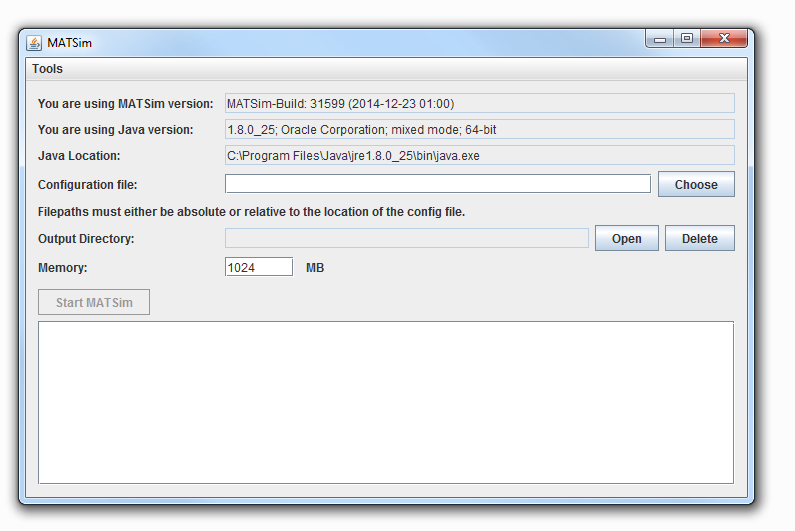
\includegraphics[width=0.8\textwidth, angle=0]{using/figures/matsimgui.png}}%
{}
% ----------

For the release 0.6, \gls{matsim} does not provide a \gls{gui}, thus, you need to be able to handle and access a command line tool.\footnote{%
%
\parskip0.3\baselineskip
\parindent0pt
%
In Linux or Mac OS X, this is typically a Terminal application, and in Windows, the Power Shell or Command Prompt.
%
On the command prompt type the following command as one line, but substitute the correct paths: 
\lstinline|java -Xmx512m -cp /path/to/matsim.jar org.matsim.run.Controler /path/to/config.xml|

As an example, on Linux this could look like: 
\lstinline|java -Xmx512m -cp /path/to/matsim.jar org.matsim.run.Controler /path/to/config.xml|

On Mac OS X, it could look like this: 
\lstinline|java -Xmx512m -cp /path/to/matsim.jar org.matsim.run.Controler /path/to/config.xml|

On Windows, an example command could be: 
\lstinline{java -Xmx512m -cp C:}$\backslash$\lstinline{MATSim}$\backslash$\lstinline{matsim.jar org.matsim.run.Controler C:}$\backslash$\lstinline{MATSim}$\backslash$\lstinline{input}$\backslash$\lstinline{config.xml}
% problems with the combination of lstinline, backslash, and footnote. :-(  kai, jan'15

Such a command consists of multiple parts:
\begin{compactitem}
\item \lstinline|java| tells the system that you want to run \gls{java}.
\item \lstinline|-Xmx512m| tells \gls{java} that it should use up to 512\,\gls{mb} of memory. This is typically enough to run the small examples. For larger \glspl{scenario}, you might need more memory, e.g.,\,\lstinline|-Xmx3g| would allow \gls{java} to use up to 3\,\gls{gb} of \gls{ram}.
\item \lstinline|-cp /path/to/matsim.jar| tells Java where to find the \gls{matsim} code.
\item \lstinline|org.matsim.run.Controler| specifies which class (think of an "entry point") should be run. In most cases, the default \gls{matsim} \lstinline|Controler| is the class you will need to run simulations.
\item \lstinline|/path/to/config.xml| tells \gls{matsim} which \gls{configfile} is to be used. 
\end{compactitem}

}


% ================================================================================================
\subsection{Configuring \protect\gls{matsim}}
\label{sec:config}
Configuring \gls{matsim} is 
%(at this stage) only 
% KISS.  kai, jan'15
done via the \gls{configfile}. It builds the connection between the user and \gls{matsim}. It contains a list of settings which influence how the simulation behaves.
%% In the second part of the book we will learn how \gls{matsim} can be configured and extended by programming against its API. \kai{Andreas, hier brauchen wir eine Entscheidung.  Derzeit enthält ``extending matsim'' auch Material, welches alleine durch die Config angesprochen werden kann, ohne contrib und ohne programming.  Beispiele sind time-dep network, andere strategy modules, oder observational modules.  Mit ``transit'' wird das nochmal deutlich mehr.  Nichts davon ist somit ``programming against its API''.  Möglichkeiten aus meiner Sicht: 
% (1) Wir verstehen unter ``extending'' auch solche Dinge, die alleine durch die config (und evtl. zusätzliche Input-Dateien) angesprochen werden können.  
% (2) Wir packen Dinge, die über die config ansprechbar sind, aber zusätzliche Dateien benötigen, nach ``extending'', alles andere nach ``using''.  
% (3) Wir packen \emph{nur} die Dinge, bei denen man programmieren muss, nach ``extending''. --  Im Moment ist es m.E.\ (1).  -- Wenn es (1) oder (2) sind/werden, müsste man obigen Satz anpassen.}
%
\kai{Habe einen Satz, der eine Vorschau auf Part~II gibt, mal rausgestrichen.  Part~II enthält auf jeden Fall auch (viele) Dinge, die man machen kann, ohne dass man programmiert.}
\ah{Die nur grob definierte Einteilung machte mir im Modules-Chapter auch schon grosse Bauchschmerzen.

Grundidee war mal (3). Doch dann landet viel zu viel, was den Anfänger überfordert in Teil I. Das Modules-Kapitel müsste komplett auseinandergerissen werden.
(1) ist noch keine klare Grenze, was wir im Moment ja auch nicht haben. 
So was wie (2) müsste es m.E. sein, um eine didaktisch sinnvolle Einteilung zu haben. Aber auch hier, muss das Modules-Kapitel auseinandergerissen werden. Wir sollten wohl noch ein Using-Kapitel einfügen mit dem Titel "Configuring MATSim" o.ä., und da alles reinpacken, was momentan im Modules-Kapitel nur über Config angesprochen werden kann.
}

All configuration parameters are simple pairs of a \gls{parameter} \lstinline|name| and a \gls{parameter} \lstinline|value|. The \glspl{parameter} are grouped into logical groups. For example, there is a group with settings related to the \lstinline|Controler| like the number of \glspl{iteration}, or there is another group with settings related to the \gls{simulation}, e.g.,\,the end time of the simulation. As shown in Chapter~\ref{ch:modules}, a whole bunch of \gls{matsim} modules can be added to \gls{matsim} and configured by specifying the respective section of the configuration file.

The list of available parameters and valid parameter values may vary from release to release. Although we try to keep this stable,
%due to
because of changes in the software, most notably by new features, settings may change. To get a list of all available settings currently available, run the following command:
\begin{lstlisting}
java -cp matsim.jar org.matsim.run.CreateFullConfig fullConfig.xml
\end{lstlisting}
%
This command will create a new \gls{configfile} \lstinline|fullConfig.xml|, which contains the full list of available parameters along with their default values. This makes it easy to see what settings are available. To use and modify certain settings, the lines with the corresponding parameters can be copied to the \gls{configfile} specific for the \gls{scenario} to be simulated and the parameter values be modified in that file. 

A fairly minimal \gls{configfile} approximately contains the following information:
\begin{xml}
<module name="network">
   <param name="inputNetworkFile" value="<path-to-network-file>" />
</module>

<module name="plans">
   <param name="inputPlansFile" value="<path-to-plans-file" />
</module>

<module name="controler">
   <param name="firstIteration" value="0" />
   <param name="lastIteration" value="0" />
</module>

<module name="planCalcScore" >
   <parameterset type="activityParams" >
      <param name="activityType" value="h" />
      <param name="typicalDuration" value="12:00:00" />
   </parameterset>
   <parameterset type="activityParams" >
      <param name="activityType" value="w" />
      <param name="typicalDuration" value="08:00:00" />
   </parameterset>
</module>
\end{xml}
A working example can be found in the \gls{matsim} directory tree (cf.~\ref{sec:settingUpMatsim}) under \lstinline{examples/tutorial/config/example1-config.xml}.

%% A minimal \gls{configfile} is shown below, specifying the minimal information that \gls{matsim} needs about demand and supply. 
In the example, supply is given by 
the network and demand is given in the plans file (typical input data produced is described in Section \ref{sec:inputdata}). 
%
The specification that the first iteration and the last iteration are the same means that no \gls{replanning} of the demand is performed.  
%
What \emph{is} executed is the mobsim, denoted as ``execution'' in Figure~\ref{fig:matsimcycle}, followed by the scoring of each executed plan's performance.
%
The scoring, in order to work, minimally needs to know all activity types that are used in the plans, and the typical duration for each such activity type.



%% \kai{Andreas, hast Du das getestet?  Wenn ich das mache, bekomme ich eine Exception \lstinline{java.lang.IllegalArgumentException: acttype "w" is not known in utility parameters (module name="planCalcScore" in the config file)}, was dann zwar formal tatsächlich kein replanning ist, aber auch kein sauberer Abbruch.}


%% \begin{xml}
%% <?xml version="1.0" ?> 
%% <!DOCTYPE config SYSTEM "http://www.matsim.org/files/dtd/config_v1.dtd"> 
%% <config> 
 
%%    <module name="network"> 
%%       <param name="inputNetworkFile" value="example/network.xml" /> 
%%    </module> 
 
%%    <module name="plans"> 
%%       <param name="inputPlansFile" value="example/population.xml.gz" /> 
%%    </module> 
%% </config>
%% \end{xml}

% ##################################################################################################################
\section{Building and Running a Basic Scenario}
\label{sec:buildingbasicscenario}
% ===============================================================================================
This section provides information on the typical input data files used for a \gls{matsim} experiment, and the standard output files generated. It presents a parsimonious example scenario and shortly explains units, conventions and coordinate systems used in \gls{matsim}. Finally some hints on practical data requirements and how to perform calibration, verification and validation are given.

% ===============================================================================================
\subsection{Typical Input Data}
\label{sec:inputdata}
Minimally \gls{matsim} needs the files
\begin{compactitem}
	\item \lstinline|config.xml|, containing the configuration options for \gls{matsim} and presented above,
	\item \lstinline|network.xml|, with the description of the (road) network, and
	\item \lstinline|population.xml|, providing information about	the travel demand, i.e.,\,the list of agents and their day plans.
\end{compactitem}

%% \kai{Andreas, eigentlich würde ich `facilities', `vehicles', und `transit' gerne nach ``extending matsim'' verschieben: (1) `facilities' kann man nur mit core matsim und config file m.E. gar nicht benutzen, (2) schedule-based pt ist ein fehler-anfälliger plug-in, mit dem man nicht gleich ``starten'' muss.  Ok?}
\kai{clean this out (facilities, pt, etc.}

With this setting, \gls{matsim} agents perform their activities on a specific \gls{link}. If further information about \glspl{activitylocation} needs to be specified, this can be done in 
\begin{compactitem}
\item \lstinline|facilities.xml|. 
\end{compactitem}
%
If \gls{matsim} \glspl{facility} are used, the agents perform their activities in a specific \gls{facility} attached to a network link.
%
\ah{Generierung von Facilities muss/kann dann in Part II auch noch untergebracht werden: 

Clearly, many modules require further information about the infrastructure, in particular about the activity locations' open times. For the Swiss scenario the facilities are derived from a business census \citep[][]{SwissEnterpriseCensus_manual_2001}. Comparable data is available in most countries from official sources, such as censuses, and commercial sources, such as navigation network providers, yellow pages publishers or business directories, and last but not least google and \gls{osm} \citep[][]{OpenStreetMap_Webpage_2015}.
}
%

In the beginning of \gls{matsim} only car mode could be simulated. With the addition of the public transport \gls{module} (Chapter~\ref{ch:pt}), with the help of two further input files public transport can just as well be simulated:
\begin{compactitem}
\item \lstinline|transitVehicles.xml| providing the description of the vehicles used for public transport services. \kai{vehicles.xml?  (without ``transit''?)} \kai{Andreas, fyi: I think we are leaning towards having separate containers vehicles.xml and transitVehicles.xml.  Not yet implemented.}
\item \lstinline|transitSchedule.xml| containing information about transit stop locations and transit services,
\end{compactitem}
%
For the handling of other modes please refer to Chapter~\ref{ch:multimodalsim}.

Count data are a common evaluation measure in transport planning. In \gls{matsim}, count data can be integrated with the file
\begin{compactitem}
\item \lstinline|counts.xml| containing hourly volumes from real-world counting stations.
\end{compactitem}

Some of the files, especially \lstinline|population.xml|, but also \lstinline|network.xml| or \lstinline|facilities.xml| \kai{chk if already known here}, might get quite large. To save space, \gls{matsim} supports reading and writing the data in a compressed format. \gls{matsim} uses GZIP-compression for this. Thus, in many cases, the file names have the additional suffix \lstinline|.gz|, as in \lstinline|population.xml.gz|. \gls{matsim} automatically detects if files are compressed or should be written compressed based on the file name.
 
In more detail, the input files look as follows. For the config file, see Section~\ref{sec:config} above. 

\makeatletter
\newcommand\thefontsize{{The current font size is: \f@size pt\par}}
\makeatother

% -----------------------------------------------------------------------
\subsubsection{\lstinline{network.xml}}
\label{sec:lgstartednetwork}



The network describes the infrastructure on which the agents (or the vehicles, respectively), can move around. The network consists of \glspl{node} and \glspl{link} (in graph theory, these are typically called vertices and edges). A simple example for a description of a network in \gls{matsim}'s \gls{xml} data format 
%can look as follows.
approximately contains the following information:
%% <?xml version="1.0" encoding="utf-8"?> 
%% <!DOCTYPE network SYSTEM "http://www.matsim.org/files/dtd/network_v1.dtd"> 
\begin{xml}
<network name="example network"> 
   <nodes> 
      <node id="1" x="0.0" y="0.0"/> 
      <node id="2" x="1000.0" y="0.0"/> 
      <node id="3" x="1000.0" y="1000.0"/> 
   </nodes> 
   <links> 
      <link id="1" from="1" to="2" length="3000.00" capacity="3600" 
            freespeed="27.78" permlanes="2" modes="car" /> 
      <link id="2" from="2" to="3" length="4000.00" capacity="1800" 
            freespeed="27.78" permlanes="1" modes="car" /> 
      <link id="3" from="3" to="2" length="4000.00" capacity="1800" 
            freespeed="27.78" permlanes="1" modes="car" /> 
      <link id="4" from="3" to="1" length="6000.00" capacity="3600" 
            freespeed="27.78" permlanes="2" modes="car" /> 
   </links> 
</network>
\end{xml}
For a working example, check the \lstinline{examples/equil} directory in the \gls{matsim} directory tree (cf.\ Section~\ref{sec:settingUpMatsim}).

Each element has an identifier \lstinline|id|. Nodes are described by an \lstinline|x| and a \lstinline|y| coordinate value. Links have more attributes: The \lstinline|from| and \lstinline|to| attribute reference nodes and describe the geometry of the network. Additional attributes describe the traffic-related aspects of the links:
%network:
\begin{compactitem}
    \item the \lstinline|length| of the link, typically in meters (see Section~\ref{sec:unitsconventions}).
    \item the flow \lstinline|capacity| of the link, i.e.,\,the number of vehicles that can pass the link, typically in vehicles per hour.
    \item the \lstinline|freespeed| is the maximum speed at which vehicles are allowed to travel along the link, typically in meters per seconds.
    \item the number of lanes (\lstinline|permlanes|) available in the direction specified by the from and to nodes.
    \item the list of \lstinline|modes| allowed on the link. This is a comma-separated list, e.g.,\,\lstinline|modes="car, bike, taxi"|.
\end{compactitem}
%Note that
All links are uni-directional. If a road can be traveled in both directions, two links have to be defined with alternating \lstinline|to| and \lstinline|from| attributes (see links with id 2 and 3 in the example given in the listing above). Thus, the network can be seen as a directed graph. 

% -----------------------------------------------------------------------
\subsubsection{\lstinline|population.xml|}
\label{sec:lgstarted-population}

\paragraph{File format}

The travel demand for \gls{matsim} is described by the agents' day plans. The full set of agents is typically the population, hence the file name \lstinline|population.xml|. Alternatively, \lstinline|plans.xml| is also commonly used in \gls{matsim}, as the population file essentially contains a list of day plans.

The population contains the data in a hierarchical structure as shown in the following small example.  This example is meant to illustrate the data structure; minimal input files can do with less information, see a bit later.
%% <?xml version="1.0" encoding="utf-8"?> 
%% <!DOCTYPE population SYSTEM "http://www.matsim.org/files/dtd/population_v5.dtd"> 
\begin{xml}
<population> 
   <person id="1"> 
      <plan selected="yes" score="93.2987721"> 
         <act type="home" link="1" end_time="07:16:23" /> 
         <leg mode="car"> 
            <route type="links">1 2 3</route> 
         </leg> 
         <act type="work" link="3" end_time="17:38:34" /> 
         <leg mode="car"> 
            <route type="links">3 1</route> 
         </leg> 
         <act type="home" link="1" /> 
      </plan> 
   </person> 
   <person id="2"> 
      <plan selected="yes" score="144.39002"> 
         ...
      </plan> 
   </person> 
</population>
\end{xml}
For a working example, check the \lstinline{examples/equil} directory in the \gls{matsim} directory tree (cf.\ Section~\ref{sec:settingUpMatsim}).

The population contains a list of persons, each person contains a list of plans, and each plan contains a list of activities and legs.

Exactly one \gls{plan} per person is marked as selected. The selected plan of each agent is the plan that gets executed by the mobility simulation. During the \gls{replanning} stage, a different plan might get marked as being selected. A \gls{plan} can contain a score as attribute. The score gets calculated and stored in the plan during the scoring stage, after the plan was executed by the mobility simulation.

The list of activities and legs in each plan describe the planned actions by each agent. Activities have a type assigned and have---except for the last activity in a day plan---an end time defined (there are some exceptions where activities have a duration instead of an end time. Such activities are often automatically generated by routing algorithms and are thus not described in this guide). To describe the location where an activity takes place, the activity is either assigned a coordinate by giving an \lstinline|x| and \lstinline|y| attribute value, or has a link assigned which describes from which link the activity can be reached. As the simulation requires the link attribute, the \lstinline|Controler| calculates the nearest link for a given coordinate in the case the attribute is missing and only an \lstinline|x| and \lstinline|y| coordinate value is given or any activity.

A \gls{leg} describes how agents plan to travel from one location to the next one. Each \gls{leg} must have a transport mode assigned. Optionally, legs may have an attribute \lstinline|trav_time| which describes the expected travel time for this leg. For a leg to be simulated, it must contain a route. The format of a route depends on the mode of a leg. For car-legs, the route lists the links that the agent has to travel along in the given order, while for transit-legs information about the stop locations and expected transit services are stored.

An agent starts a leg directly after the previous activity (or leg) has ended. Depending on the mode, the \gls{mobsim} might handle the agent differently. By default, car- and transit-legs are well-supported by the \gls{mobsim}. If the \gls{mobsim} encounters a mode it does not know, it defaults to \gls{teleportation}: In this case, the agent is removed from the simulated reality, and after the leg's expected travel time has passed, re-inserted at the agent's target location.

\paragraph{A minimal populations file}

The population data format is one of the most central data structures in \gls{matsim} and might be a bit overwhelming at first. Luckily, to get started, only a small subset must be known of it.  A population file approximately needs the following information:
%% The following listing shows how a minimal population file could look like. 
%% <?xml version="1.0" encoding="utf-8"?> 
%% <!DOCTYPE population SYSTEM "http://www.matsim.org/files/dtd/population_v5.dtd"> 
\begin{xml}
<population> 
   <person id="1"> 
      <plan> 
         <act type="home" x="5.0" y="8.0" end_time="08:00:00" /> 
         <leg mode="car" /> 
         <act type="work" x="1500.0" y="890.0" end_time="17:30:00" /> 
         <leg mode="car" /> 
         <act type="home" x="5.0" y="8.0" /> 
      </plan> 
   </person> 
   <person id="2"> 
      ... 
   </person> 
</population>
\end{xml}
For a working example, check the \lstinline{examples/equil} directory in the \gls{matsim} directory tree (cf.\ Section~\ref{sec:settingUpMatsim}).

Notably, the following simplifications can be made:
\begin{compactitem}
\item Each person needs exactly one plan.
\item The plan does not need to be selected or have a score.
\item Activities can be located just by their coordinates.
\item Activities should have a somewhat meaningful end-time.
\item Legs only need a mode, but no routes.
\end{compactitem}
When a simulation is started, \gls{matsim}'s \lstinline|Controler| will load such a file and then automatically assign the nearest link to each activity and calculate a suitable route for each leg. This makes it easy to get started quickly. 

% -----------------------------------------------------------------------
\subsubsection{\lstinline|counts.xml|}
\gls{matsim} provides funtionality to compare traffic volumes from your simulation to real world values. The Counts infrastructure allows to compare the traffic volumes on links on an hourly basis. The following listing shows an example of a \lstinline|counts.xml| input file required to do traffic count comparisons. 

\begin{xml}
<?xml version="1.0" encoding="UTF-8"?> 
<counts xmlns:xsi="http://www.w3.org/2001/XMLSchema-instance" 
        xsi:noNamespaceSchemaLocation="http://matsim.org/files/dtd/counts_v1.xsd" 
        name="test" desc="test counting stations" year="2014"> 
   <count loc_id="2" cs_id="005"> 
      <volume h="1" val="10.0"></volume> 
      <volume h="2" val="1.0"></volume> 
      <volume h="3" val="2.0"></volume> 
      <volume h="4" val="3.0"></volume> 
      <volume h="5" val="4.0"></volume> 
      <volume h="6" val="5.0"></volume> 
      <volume h="7" val="6.0"></volume> 
      <volume h="8" val="7.0"></volume> 
      <volume h="9" val="8.0"></volume> 
      <volume h="10" val="9.0"></volume> 
      <volume h="11" val="10.0"></volume> 
      <volume h="12" val="11.0"></volume> 
      <volume h="13" val="12.0"></volume> 
      <volume h="14" val="13.0"></volume> 
      <volume h="15" val="14.0"></volume> 
      <volume h="16" val="15.0"></volume> 
      <volume h="17" val="16.0"></volume> 
      <volume h="18" val="17.0"></volume> 
      <volume h="19" val="18.0"></volume> 
      <volume h="20" val="19.0"></volume> 
      <volume h="21" val="20.0"></volume> 
      <volume h="22" val="21.0"></volume> 
      <volume h="23" val="22.0"></volume> 
      <volume h="24" val="23.0"></volume> 
   </count> 
</counts>
\end{xml}
For a working example, check the \lstinline{examples/equil} directory in the \gls{matsim} directory tree (cf.\ Section~\ref{sec:settingUpMatsim}).

It starts with a header containing general descriptive information about the counts, including a year to describe how current the data is. Next, for each link having real world counts data, the hourly volumes can be specified. The network-link is referenced by the \lstinline|loc_id| attribute, in the example, it is link 2. The attribute \lstinline|cs_id| (counting station identifier) can be used to store an arbitrary description of the counting station. Most often it is used to note the original real word counting station to simplify future data comparison. The hourly volumes, specified by the hour of the day and its value, are optional: That is, not for every hour a value must be given. If for a counting station data is only available for certain hours of the day (e.g.,\,only during peak hours) it is possible to omit the other hours from the \gls{xml} listing.  Note that the first hour of the day, from 0:00 to 1:00, is numbered as ``1'', and \emph{not} by ``0'' as is often done in computer science.

% ===============================================================================================
\subsection{Typical Output Data}
\label{sec:outputdata}
\gls{matsim} creates
%a bunch of
output data, which can be used to analyze the results but also to monitor the correct working of the current simulation setup. Some of the files summarize a complete \gls{matsimrun}, while others are created for a specific \gls{iteration} only. The first ones go directly to the top level of the output folder, which can be specified in the \lstinline|controler| section of the config file. The latter ones are stored in iteration-specific folders \lstinline|ITERS/it.{iteration number}| continuously created in the output folder. For some files (typically for the large ones, such as the population) the output frequency can be specified in the \gls{configfile}. They go to the respective iteration folder. The files that summarize the complete \gls{matsimrun} are built up on the fly, i.e.,\,after every iteration the currently computed iteration values are stored, such that a continuous monitoring of the run is possible. There are files that are created by default (such as the score statistics files) and there are files that need to be triggered by a respective configuration file section (such as count data files).

%\kai{Sollten wir (1) den Unterschied zwischen ``main'' und ``ITERS'' directory beschreiben, und (2) darauf hinweisen, wo die folgenden Dateien jeweils sind?}
%\ah{sollte jetzt erledigt sein}

The following output files are continuously built up to summarize the complete run.
\begin{description}

  \item[Log File:]
During a \gls{matsimrun}, a log file is printed. This file contains information that you might need later for your analyses. Additionally, it might be helpful if a run has crashed for some unknown reason. 

\item[Warnings and Errors Log File:]
Sometimes, \gls{matsim} recognizes problems in the simulation or the configuration of it. It will then write warnings and errors to the log file. As the log file contains a lot of information, such warnings might get overlooked. For this reason, a separate log file is generated in the output directory of a run containing only warnings and error messages. It is advised to have a look during/after a run into this file to see if there have been any major problems.

\item[Score Statistics:]
Score statistics are available as picture (\lstinline|scorestats.png|) as well as a text file (\lstinline|scorestats.txt|). They show the average best, worst, executed and average of all plans of an agent for every iteration. An example score plot is shown in Figure~\ref{fig:scoreprogress}.

\item[Leg Travel Distance Statistics:]
Leg travel distance statistics are comparable to the score statistics, but instead of the score, the travel distance is plotted. The files are named \lstinline|traveldistancestats.png| and \lstinline|traveldistancestats.txt|.

\item[Stopwatch:]
The stopwatch file (\lstinline|stopwatch.txt|) contains the computer time (so-called wall clock time) of actions like the replanning or the execution of the mobility simulation for every iteration. This data might be helpful for performance analyses (e.g.,\,how long does the replanning take compared to the mobility simulation?).

\end{description}

%\kai{``run'' vs ``iterations'': Wir benutzen normalerweise die Semantik, dass ein ``run'' die Summe aller ``iterations'' ist.  Dann wäre das oben ``Once per iteration''.  Oder ``At the end of each run'', obwohl das technisch nicht richtig ist, weil es tatsächlich am Ende einer jeden Iteration neu erzeugt wird; so kann man alles bereits während der Iterationen mitverfolgen.}
%\ah{sollte jetzt erledigt sein}

The following output files are created for specific iterations:
\begin{description}

\item[Events:] Every action in the simulation is recorded as a so-called \gls{matsim} \gls{event}, be it the starting of an activity or the change of a network link. Each \gls{event} hosts one or multiple attributes. By default, the time when the \gls{event} occurred is contained. Additionally, information like the id of the agent who caused the event or the id of the link where the \gls{event} occurred could be included. By default, the \gls{matsim} simulation module creates a so called events-file in every 10th iteration. This file contains every single \gls{event} that has been created by the simulation. The events file is thus a formidable base for post-analyses for example with the visualizers. Events are discussed in detail in Section~\ref{sec:events-extension-point}.

\item[Plans:] At configurable iterations the current state of the population with the agents' plans is printed.
%
The final iteration's plans 
%and events % nicht per default. kai, jan'15
are also generated on the top level of the output folder.

\item[Leg Histogram:]
In every iteration, a leg histogram is plotted. A leg histogram depicts the number of agents that arrive, depart or are en route per time unit. Histograms are created for each transport mode and, additionally, for the sum of all transport modes. Each file starts with the iteration number and ends with the transport mode (e.g.,\,\lstinline|1.legHistogram_car.png| or \lstinline|1.legHistogram_all.png|). Moreover, a text file is created (e.g.,\,\lstinline|1.legHistogram.txt|) that contains the data for all transport modes.

\item[Trip Durations:]
Per iteration, a \gls{trip} durations text file (e.g.\ \lstinline|1.tripdurations.txt|) listing the number of trips and their durations on a time bin level for each activity pair (e.g.,\,from work to home or from home to shopping) is put out.

\item[Link Volumes:]
The printing of the link volume comparison (between simulated and counted volumes) needs to be triggered by a config file entry. The comparison generates overview summaries for the whole network but also analyses for individual links. A link analysis might look like Figure~\ref{fig:countcomparison}.

\end{description}

% ----------
\createfigure%
{Example for a link volumes comparison between simulation and road count values}%
{Example for a link volumes comparison between simulation and road count values}%
{\label{fig:countcomparison}}%
{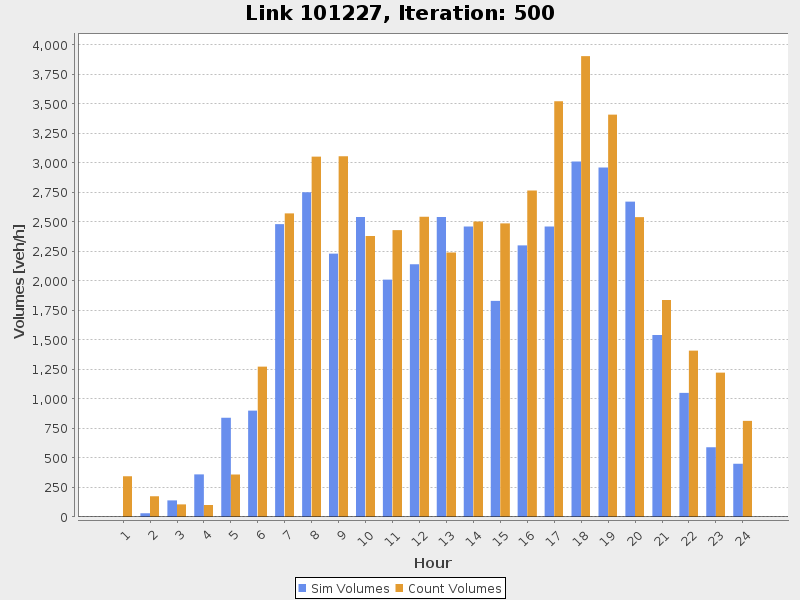
\includegraphics[width=0.7\textwidth, angle=0]{using/figures/link101227.png}}%
{}
% ----------

% ===============================================================================================
\subsection{An Example Scenario}
The \gls{matsim} release is shipped with an example scenario named \lstinline|equil| in the folder \lstinline|examples/equil|. The scenario contains the following files \lstinline|config.xml|, \lstinline|network.xml| and \lstinline|plans100.xml|, \lstinline|plans2000.xml.gz| containing 100 and 2000\,persons respectively with their day plans using the car mode only. A tiny population containing only 2\,persons (\lstinline|plans2.xml|) one using public transport, the other person using car mode, is also provided. Furthermore, an example for count data can be found in the folder (\lstinline|counts100.xml|). 

%% or trips with taxi mode is also provided (\lstinline|plans-w-taxi.xml|). 
%% A tolls file can be used for road pricing scenarios not discussed here (\lstinline|toll.xml|).

%\kai{Habe da neulich, als Resultat einer Diskussion, etwas ausgedünnt.  Müssen wir ggf.\ anpassen, aber m.E.\ stimmt es so nun.}
%\ah{https://matsim.atlassian.net/browse/MATSIM-286}

There is also a file with a demand of 
%exactly 
% KISS.  kai, jan'15
100~\emph{trips} (\lstinline|plans100trips.xml|), i.e.,\,demand just going from one location to another, using a \lstinline$dummy$ activity type at each end.  This is provided to show that \gls{matsim} can also be run as a fully trip-based approach, i.e.\ completely without considering activities. Clearly, it loses some of its expressiveness, but the basic concepts, including route and even departure time adaptation, still work in exactly the same way.

The network of the scenario is shown in Figure~\ref{fig:equil}.

% ----------
\createfigure%
{Equil scenario network}%
{Equil scenario network}%
{\label{fig:equil}}%
{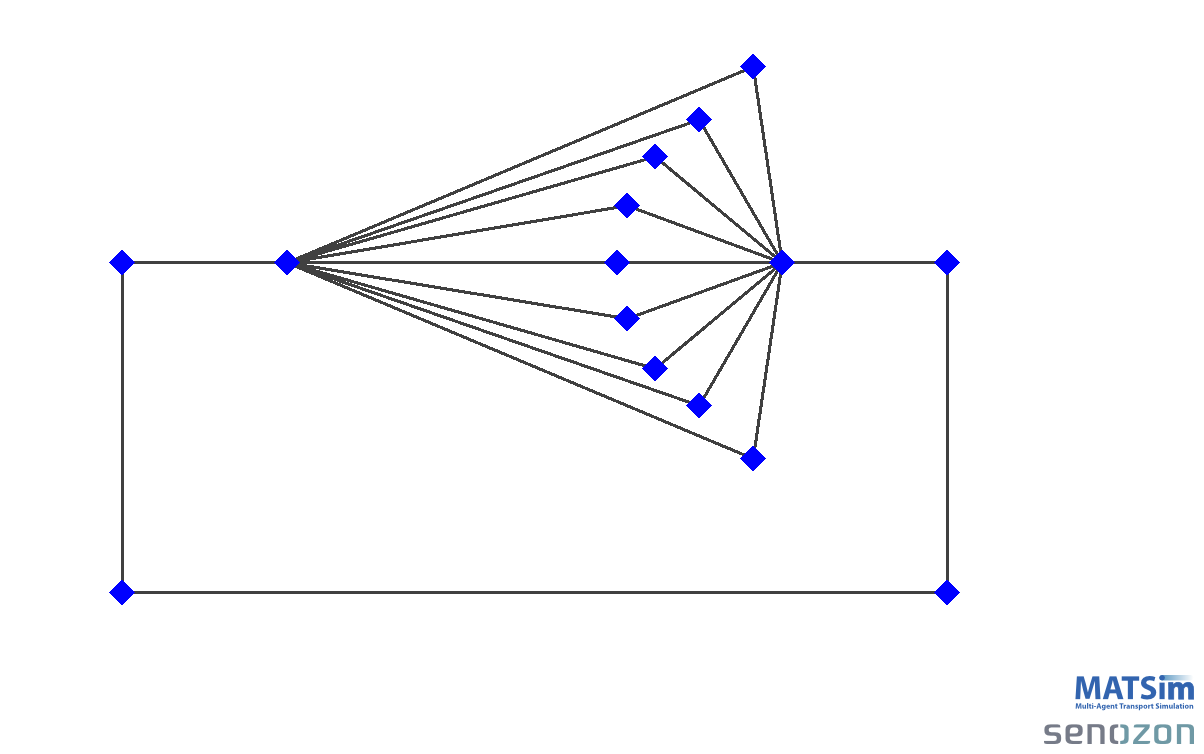
\includegraphics[width=0.8\textwidth, angle=0]{using/figures/equil.png}}%
{}
% ----------

The following lines explain the scenario by picking and discussing most important sections from the config file \lstinline|config.xml|.


\paragraph{``strategy'' section of the config file}

As shown in the listing below, this scenario uses replanning. 10\,\% of the agents reroute their current route (module \lstinline|ReRoute|). The remaining 90\,\% select their highest score plan for re-execution in the current iteration (module \lstinline|BestScore|). Plans get deleted from the agent's memory if it is full defined by \lstinline|maxAgentPlanMemorySize|. By default, the plan with the lowest score is removed, while this is configurable and currently subject of
%intense % kein funding. kai, jan'15
research (see Section~\ref{sec:choicesets}).
%
\begin{xml}
<module name="strategy">
	<param name="maxAgentPlanMemorySize" value="5" /> <!-- 0 means unlimited -->
	
	<parameterset type="strategysettings" >
		<param name="strategyName" value="SelectExpBeta" />
		<param name="weight" value="0.9" />
	</parameterset>
	
	<parameterset type="strategysettings" >
		<param name="strategyName" value="ReRoute" />
		<param name="weight" value="0.1" />
	</parameterset>
	
</module>
\end{xml}


%% \kai{I think there is a better syntax for the above now (without the numbering); should we use that?}
%% \ah{ersetzt}

\paragraph{``planCalcScore'' section of the config file}

The section \lstinline|planCalcScore| defines the parameters used for scoring. The parameters are explained in Chapter~\ref{ch:scoring}. As can be seen in the example, the two activity types \lstinline|h| (home) and \lstinline|w| (work) are specified.  All activity types contained in the population file (cf.~Section~\ref{sec:lgstarted-population}) need to be defined in the \lstinline{planCalcScore} section of the config file.
\begin{xml}
<module name="planCalcScore" >
   <parameterset type="activityParams" >
      <param name="activityType" value="h" />
      <param name="typicalDuration" value="12:00:00" />
   </parameterset>
   <parameterset type="activityParams" >
      <param name="activityType" value="w" />
      <param name="typicalDuration" value="08:00:00" />
   </parameterset>
</module>
\end{xml}

\paragraph{``controler'' section of the config file}

The scenario is run for 10\,iterations, writes the output files to \lstinline|./output/equil| (Section~\ref{sec:outputdata}), and uses \gls{qsim} as the mobility simulation (more on \glspl{mobsim} in Section~\ref{sec:trafficflowmodel} and \ref{sec:mobsims}).
\begin{xml}
<module name="controler">
	<param name="outputDirectory" value="./output/equil" />
	<param name="lastIteration" value="10" />
	<param name="mobsim" value="qsim" />	
</module>
\end{xml}

%% \kai{I would suggest to say something about via already at this point.  There is a free educational version so I think that this would be ok.}
%% \ah{ok}

\paragraph{Visualization}

Simulation results can be comfortably analyzed using one of the visualizers, via (Chapter~\ref{ch:via}) or OTFVis (Chapter~\ref{ch:otfvis}).

% ===============================================================================================
\subsection{Units, Conventions, and Coordinate Systems}
\label{sec:unitsconventions}
% ----------------------------------------------------------------------------
\subsubsection{Units}
\gls{matsim} tries to make as few assumptions about actual units as is possible, but at some places it cannot be done without any. In general, \gls{matsim} expects similar values (e.g.,\,all distances) to be in the same unit wherever they are used. In the following, the most important (expected) units are listed in a short overview. 

% .......................................................
\paragraph{Distance}

Distance units are most prominently used in links' length. They should be specified in the same unit that the coordinate system uses. This allows \gls{matsim} to use simple triangulation, e.g.,\,with the nodes' coordinates, to calculate beeline distances. As most of the typically used, projected coordinate systems (see Section~\ref{sec:coordinatesystems}) use meters as unit of distance, this is the most common used unit of distance in \gls{matsim}. 

% .......................................................
\paragraph{Time}

While \gls{matsim} supports an hour:minute:second notation in several places, internally it uses seconds as the default time unit. This implies that for example link speeds must be specified in distance per second, typically meters per second. One notable exception from this rule are scoring parameters, where \gls{matsim} expects values per hour. This is due to the fact that most behavioral parameters like value of time are typically estimated per minute or hour, and that the corresponding values for seconds are very small and thus error prone to be configured. 

% .......................................................
\paragraph{Money}

Money is unit-free. The units are implicitly given by the marginal utility of money (cf.\ Equation~(\ref{eq:tdisutility}) below). That is when, say, one moves from Germany to Switzerland, then the parameter $\beta_c$ has to be changed from "utility per Euro" to "utility per Swiss Franc".

% ----------------------------------------------------------------------------
\subsubsection{Conventions}
\gls{matsim} makes heavy use of identifiers, short \lstinline|Id|s. These identifiers can be arbitrary strings, with the following exceptions: Ids should not contain any spaces (incl. tabs, new lines, etc) or commas, as those characters are typically used for separating different Ids from each other in \lstinline|Id| lists. 

% ----------------------------------------------------------------------------
\subsubsection{Coordinate Systems}
\label{sec:coordinatesystems}
\paragraph{Preparing Your Data in the Appropriate Coordinate System:}
In several input files, you need to specify coordinates, e.g.,\,for the nodes of the network. It is strongly suggested not to use WGS84 coordinates (i.e.,\,\gls{gps} coordinates) or any other kind of spherical coordinates (coordinates ranging from $-180$ to $+180$ in west-east direction and from $-90$ to $+90$ in south-north direction). \gls{matsim} needs to calculate distances between two points in several places of the code. The calculation of distances between spherical coordinates is very complex and potentially slow. Instead, \gls{matsim} uses the simple Pythagoras' theorem, but this requires the coordinates to be in a Cartesian coordinate system. Thus is is strongly advised to use a Cartesian coordinate system along with \gls{matsim}, preferably one where the distance unit corresponds to one meter.

Many countries and regions have custom coordinate system defined, optimized for usages in their appropriate areas. It might be best to ask some \gls{gis} specialists in your region of interest what the most commonly used local coordinate system is and use that as well for your data.

If you do not
%have any clue about what
know which coordinate system is used in your region, it might be best to use the \gls{utm} coordinate system. This coordinate system divides the world into multiple bands, each six degrees wide, and separated into a northern and southern part, which it calls \gls{utm} zones. For each zone, an optimized coordinate system is defined. Choose the \gls{utm} zone which covers your region (Wikipedia has a nice map showing the zones) and use its coordinate system. 

\paragraph{Telling MATSim about Your Coordinate System:}

For some operations, \gls{matsim} must know the coordinate system your data is in. For example, some analyses may create output to be visualized in \gls{googleearth} or by \gls{qgis}.
%, where the coordinates need to be converted back to WGS84.
The coordinate system used by your data can be specified in the \gls{configfile}:
\begin{xml}
<module name="global"> 
  <param name="coordinateSystem" value="EPSG:32608" /> 
</module>
\end{xml}
This allows \gls{matsim} to work with your coordinates and convert them whenever needed. 

You have multiple ways to specify the coordinate system you use. The easiest one is to use the so-called "\gls{epsg} codes". Most of the commonly used coordinate systems got standardized and numbered. The \gls{epsg} code uniquely identifies a coordinate system and can be directly used by \gls{matsim}. As an alternative, \gls{matsim} can also parse the description of a coordinate system in the so-called \gls{wkt} format. As the \gls{wkt} format is more error prone \kai{Andreas, gibt es eine Referenz oder einen anderen Grund dafür?  Falls nicht, dann können wir vielleicht ohne diese Empfehlung auskommen?} it is suggested to use \gls{epsg} codes whenever possible.

To find the correct EPSG code for your coordinate system (e.g.,\,for one of the \gls{utm} zones), the website \url{http://www.spatialreference.org} is of great use. Search on this website for your coordinate system, e.g.,\,for "WGS84 / \gls{utm} Zone 8N" (for the northern-hemisphere \gls{utm} Zone 8) to find a list of matching coordinate systems along with their \gls{epsg} codes.


% ===============================================================================================
\subsection{Data Requirements}
% ----------------------------------------------------------------------------
\subsubsection{Population and Activity Schedules}
Demand estimation is 
%the main 
an important purpose of \gls{matsim}. That means that---in theory---only these demand components have to be provided to \gls{matsim} that in reality typically do \emph{not} change
%during the
from one simulated average working day to the next. Examples are the population and its residential and working locations. In practice, however, \gls{matsim} is not quite there yet to endogenously model the complete travel demand. The sequence and preferred durations of activities for example have to be provided as input. In consequence all travel demand choices, which are not covered by the \gls{matsim} loop, have to be endogenously estimated. 

For population generation, basically two possibilities exist. The comfortable way is to translate full population census and the slightly more demanding way is synthetic population generation \citep[e.g.,][]{GuoBhat_TRR_2007} based on sample or structure surveys. For \gls{matsim} both ways have been implemented based on \citet[][]{BfS_VZ_2000} and \citet[][]{Mueller_unpub_STRC_2011} respectively.

The travel demand is usually derived from surveys; for Switzerland from the \gls{microcensus} \citep[][]{BfS-MZ2005_manual_2006}. Newer data sources, such as \gls{gps} or smartphone travel diaries might be an interesting future possibility.

A critical topic in demand and population generation is work place assignment, as commuting traffic is still dominant in particular in peak hours. In Switzerland's full census work location was asked at municipality level. Such comfortable data base is seldom however, and, thus, commuter matrix estimation or work place choice models should be urgently researched.

Having generated the residential population of the study area, additional demand components might need to be added, for example cross-border and freight traffic. As these components often cannot be endogenously modeled, \gls{matsim} offers the feature to handle different subpopulations differently (Section~\ref{sec:strategymodules}). It can be specified, that border-crossing agents, for example, are not allowed to do destination choice within the study area, or that freight agents are not allowed to change their delivery activity to a leisure activity.

% ----------------------------------------------------------------------------
\subsubsection{Network}
%\subsubsection{Supply Side}
%With the exception of some experimental work \citep[][]{HorniEtAl_TechRep_IVT_2012}, supply side is not changed by \gls{matsim}. \kai{Andreas, what about 
%\begin{itemize}
%\item network change events
%\item signals
%\item emissions/exposure internalization durch roadpricing (m.E.\ ist die Bepreisung des supplies immer noch eine supply side decision)
%\item Andreas Neumann minibus contrib
%\item Taxis (ist das demand side oder supply side?)
%\end{itemize}
%Ich bin ja ohnehin kein großer Anhänger dieser demand/supply side Unterscheidung; sollten wir hier nicht lieber einfach ``network'' in die Überschrift schreiben?}  
%
%\ah{Hab dann auch gleich die Facility Info verschoben}
%
In simulation practice, two different network types are in use, planning networks and navigation networks (compare the Swiss examples in Figure~\ref{fig:planningnetwork} and Figure~\ref{fig:navigationnetwork} for the Zürich region). The former are thinned out and serve for initial explorative simulation runs, while the later are used for policy runs usually offering much more details such as bike and even pedestrian links. Data are available from official sources like federal offices, free sources, such as \gls{osm} \citep[][]{OpenStreetMap_Webpage_2015}, and commercial sources, such as navigation network providers.
%
\createfigure%
{Zürich networks}%
{Zürich networks}%
{\label{fig:zhnetwork}}%
{%
  \createsubfigure%
  {Planning network}%
  {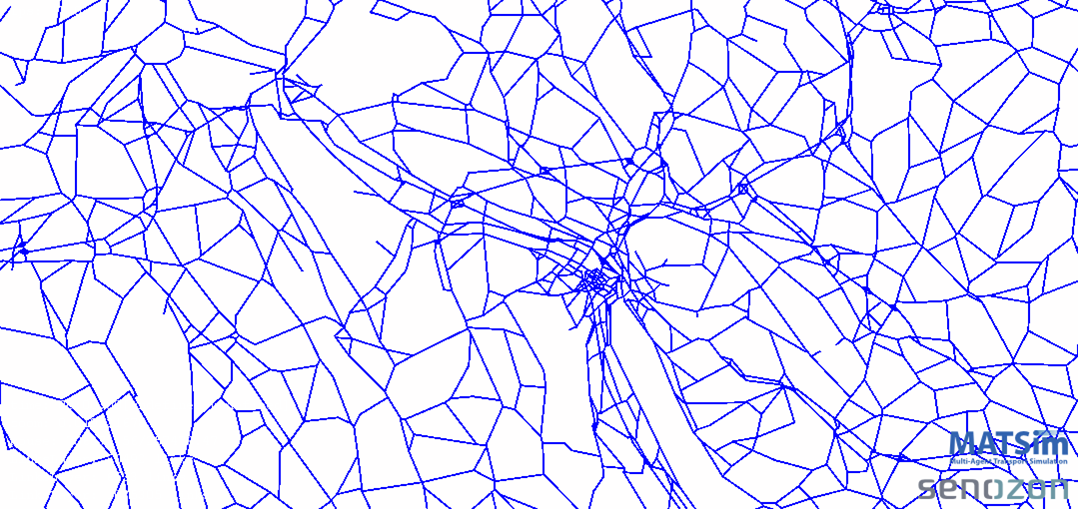
\includegraphics[width=0.8\textwidth,angle=0]{using/figures/planning.png}}%
  {\label{fig:planningnetwork}}%
  {}%
  \createsubfigure%
  {Navigation network}%
	{
\includegraphics[width=0.8\textwidth,angle=0]{using/figures/navigation.png}}%
  {\label{fig:navigationnetwork}}%
  {}%
}%
{}

% ===============================================================================================
\subsection{Calibration, Verification, and Validation}

\ah{see calibration mail by Kai}

Calibration is a necessary task of any simulation study. Main calibration component is the \gls{utilityfunction}; it needs to reflect the preferences of the study area's population. A second prominent calibration screw is used for sample \glspl{scenario}. To reduce the computational effort, initial explorative simulation runs are often performed as sample runs. In this case either the flow and storage capacity values of the mobility simulation or the network capacities need to be adapted accordingly.

Verification and validation, however, are of more concern for the \gls{microsimulation} developers. Given a valuable estimate for demand and supply including a properly estimated utility function, from customer's perspective the simulation can be expected to generate valuable single run results out of the box.

The user's or customer's responsibility is asked, at another place, though. \Glspl{microsimulation} are basically a sampling tool, just as a survey (see Section~\ref{sec:variability}). A single run represents the sampling unit, the individual in surveys. This obviously means that \gls{microsimulation} results must not to be presented as single runs but with the help of the usual statistical tools, e.g.,\,by parameters with the common measures of spread or confidence intervals. That basically means that the user/customer is responsible to specify the sample size, the number of simulation runs initialized with different random seeds. 

Policy evaluations are often based on count data, usually widely available but also showing substantial temporal variability. For \gls{matsim}, the count data need to be converted to match the simulated period of the day.

As simulation practice often mixes the terms, a few more theoretical words are said hereabout calibration, verification and validation. 

These crucial steps are located in the modeling process as sketched in Figure~\ref{fig:modeling}, which is loosely based on \citet[][Figure 10.2]{Petty_SokolowskiBanks_2010}. 

\emph{Calibration} is the process of adjusting model parameters to increase consistency of model outputs and observed target values \citep[][p.348]{HollanderLiu_Transportation_2007} \citep[see also][]{TrucanoEtAl_RESS_2006}. \citet[][Table 1]{HollanderLiu_Transportation_2007} list numerous studies that each calibrate a specific transport microsimulation. Further examples are \citet[][]{SmithEtAl_JTE_2008, KimEtAl_TRR_2005, RutterEtAl_JASA_2009}, microsimulation calibration guidelines are provided by \citet[][]{MilamChao_TRBATPM_2001, WegmannEverett_TechRep_CTRUT_2008, DowlingEtAl_manual_2002}. \citet[][Table 2]{HollanderLiu_Transportation_2007} describe measures of goodness-of-fit, that are productive for calibration. Due to the usually large number of model parameters, an automated process is favorable as far as possible. Essentially this is an optimization process \citep[][p.353]{HollanderLiu_Transportation_2007}, for which various established procedures exist \citep[e.g.,][p.41ff]{ZhangMa_ResRep_PATH_2008}. For \gls{matsim}, an automatic procedure adapting the plans to road counts was developed by \citet[][]{floetteroed-2010e}. It is unclear however, if a certain loss of behavioral soundness is caused by adapting plans according to statistical matching. On the other hand, it is unclear anyway, to date, if the \gls{matsim} relaxation transitions should be given a behavioral meaning.

Verification is the procedure to test if a "\emph{product is consistent with its specifications [...]}" \citet[][p.330]{Petty_SokolowskiBanks_2010}. In verification, a perfect match can be achieved comparing the conceptual and the executable model (see Figure \ref{fig:modeling}) in contrast to validation, where the model is always an approximation to reality \citep[][p.145]{Kleijnen_EJOR_1995}. According to \citet[][p.331]{Petty_SokolowskiBanks_2010}, "\emph{validation is the process of determining the degree to which the model is an accurate representation of the simuland.}" Validation is difficult to standardize due to the variety of models and model purposes. Some measures, tests, and applications relevant to transport modeling are given by \citet[][Table 2]{MilamChao_TRBATPM_2001}, \citet[][]{Lima_TechRep_LMPO_2006}, \citet[][p.155]{KurthEtAl_TRBTDF_2006}, \citet[][p.157]{PendyalaBhat_TRBTDF_2006}, \citet[][p.8]{WegmannEverett_TechRep_CTRUT_2008}, \citet[][]{MilamChao_TRBATPM_2001, RoordaEtAl_TransResA_2008, HawasHameed_TPT_2009, SadekEtAl_TRR_2003, GouliasKitamura_TRR_1992}, \citet[][p.25]{CambridgeSystematics_manual_2008}, \citet[][p.145]{Kleijnen_EJOR_1995} (see also \citet[][]{David_EACSSS_2009}, \citet[][p.56]{SbaytiRoden_ResRep_AASHTO_2010}, \citet[][]{SchifferRossi_TRB_2009}). While for the 4-step procedure some validation standards have emerged \citep[e.g.,][]{BartonAschmanCambridgeSystematics_manual_1997}, a lack of standardization exists for activity-based models. \citet[][]{PendyalaBhat_TRBTDF_2006} say that "\emph{despite the appeal of these models,}" [activity- and tour-based travel demand modeling systems] \emph{"their widespread implementation appears to be hindered by the absence of a detailed validation and assessment of this new wave of model systems. Many MPOs will not adopt such models until they are tested.}" \citet[][]{KurthEtAl_TRBTDF_2006} cites a statement made by Chandra Bhat and Frank Koppelman in a DRCOG e-mail discussion: "\emph{Researchers and practitioners have not thought carefully enough about the criteria for validation of models. Researchers have the habit of asking practitioners to believe that activity- based methods will produce better impact assessment and forecasts because such models more appropriately represent the actual decision process (we plead guilty to this charge). There is a good basis for this line of thought, but researchers need to go beyond this argument. They need to develop clear validation criteria and demonstrate the value of activity-based methods in ways that are easily understood.}"

Often neglected, but important, is performing sensitivity analysis (sometimes dubbed "what-if analysis" \citep[][p.155]{Kleijnen_EJOR_1995}) \citep[][]{KurthEtAl_TRBTDF_2006, CambridgeSystematics_manual_2008, CFD_TRB_2007}. Sensitivity analysis is similar to assessing elasticity of a variable \citep[][p.3f]{WegmannEverett_TechRep_CTRUT_2008} and it tests reaction of the model to changed parameters including model input. This includes both testing the range of parameters for a given point in time, and analysis of the system's fore- and backcasting abilities \citep[e.g.,][p.56]{CFD_TRB_2007}, \citep[][]{CambridgeSystematics_manual_2008}. As forecasting is a vital objective of most transport models, this test is crucial. \citet[][p.158]{PendyalaBhat_TRBTDF_2006} puts it succinctly: "\emph{There is no doubt that any model can be adjusted, refined, tweaked, and---if all else fails---hammered to replicate base-year conditions.}" and concludes that "\emph{the quality of a travel demand model system is better judged on its ability to respond to a range of scenarios and policies of interest.}" In \gls{matsim}, a natural and interesting sensitivity test would be to compare the \gls{matsim} forecasts with the current actual state of Zürich network after addition of the bypass "Westumfahrung" in 2009 \citep[][]{BalmerEtAl_ResRep_bdktzrh_2009, Westumfahrung_Webpage_2008}.

As mentioned above, models are in general flexible enough to be calibrated to target data. Thus, validation \emph{must} be performed using a different data set than for preceding modeling steps \citep[][p.1]{CambridgeSystematics_manual_2008}, \citep[][p.56]{CFD_TRB_2007}, \citep[][p.18]{OrtuzarWillumsen_2001}. In statistics, this is called cross-validation. It is particularly important for forecasting models, which need to be general enough to capture temporal changes. Calibration and validation should thus be strictly separated, however, in microsimulation practice, according to the author's opinion, they are (too) often mixed, sometimes due to the vast amount of data required for model implementation and calibration. In \gls{matsim}, for example, after model calibration only road count data is left for validation \citep[][]{HorniEtAl_STRC_2009}. New data sources, such as road speed analyses based on GPS \citep[][]{HackneyEtAl_JGS_2007}, should be included.

Having said that, validation of a large-scale transport simulation is very difficult. Many central and comfortable characteristics of systems known from natural sciences are only seldom available for the social science, such as path-independence, decomposability, isolation, and on top of that repeatability of experiments. As a result, there is still a debate if social science actually can provide something similar as laws. \citet[][p.107ff]{Abel_1976} lists and discusses the 12\,claims of the "\emph{Verstehen Position}"; although, he finds contrary arguments to every claim, nevertheless, something definitely remains true, making social science model validation exceptionally difficult. For microsimulation results interpretation and model validation, it helped me to visualize the following example. A microsimulation forecast (or backcast) regarding the construction of the "Westumfahrung Zürich" provides a probability distribution of scenarios, and it is essentially an exercise in Monte Carlo sampling (see also Chapter~\ref{ch:montecarlo}). 4\,years later we have exactly one actual state, and there is no way to assess the forecasted (or backcasted) probability distribution beyond checking that this actual state is contained in the probability distribution, and hopefully with high probability. There is nothing like Monte Carlo sampling when it comes to aggregate real system states. In other words the existing state is \emph{unique}. In essence, we thus compare an observed Dirac impulse with a computed probability distribution, which is a difficult undertaking.

% ----------
\createfigure%
{Modeling process}%
{Modeling process: Modeling starts with observation and measurement of reality (in \citet[][]{Petty_SokolowskiBanks_2010} called "\emph{simuland}") for acquisition of knowledge (in \citet[][]{Petty_SokolowskiBanks_2010} called "\emph{referent}"). Model creation---in a strict sense usually referred to as \emph{modeling}---is based on the modeler's knowledge about the world. Based on a conceptual model, an executable model is implemented and calibrated. The executable model is evaluated in a verification step in terms of "\emph{was the model made right?}" \citep[][p.332]{Petty_SokolowskiBanks_2010}. Validation compares results with the referent in the sense of "\emph{was the right model made?}" \citep[][p.332]{Petty_SokolowskiBanks_2010}.}%
{\label{fig:modeling}}%
{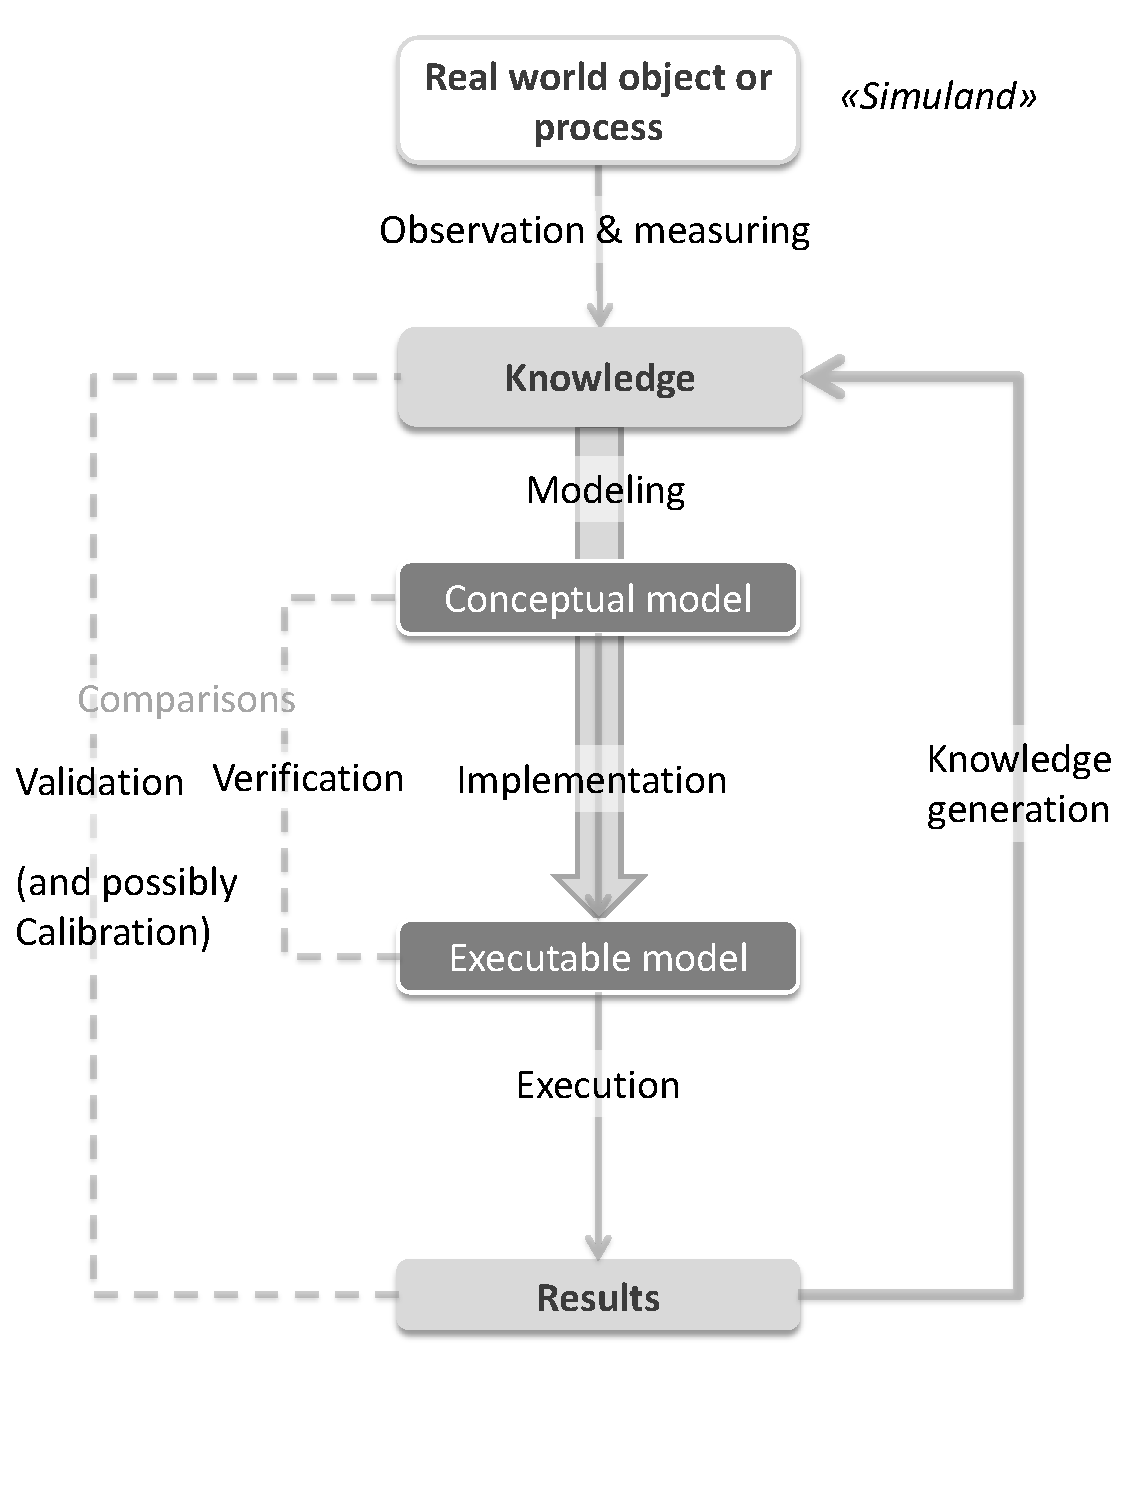
\includegraphics[width=0.8\textwidth, angle=0]{using/figures/modeling.pdf}}%
{}
% ----------

% ##################################################################################################################

% Local Variables:
% mode: latex
% mode: reftex
% mode: visual-line
% TeX-master: "../main"
% comment-padding: 1
% fill-column: 9999
% End: 
